% $Header: /cvsroot/latex-beamer/latex-beamer/solutions/generic-talks/generic-ornate-15min-45min.en.tex,v 1.5 2007/01/28 20:48:23 tantau Exp $

\documentclass[12pt]{beamer}
%\documentclass[12pt,handout]{beamer}

% This file is a solution template for:

% - Giving a talk on some subject.
% - The talk is between 15min and 45min long.
% - Style is ornate.



% Copyright 2004 by Till Tantau <tantau@users.sourceforge.net>.
%
% In principle, this file can be redistributed and/or modified under
% the terms of the GNU Public License, version 2.
%
% However, this file is supposed to be a template to be modified
% for your own needs. For this reason, if you use this file as a
% template and not specifically distribute it as part of a another
% package/program, I grant the extra permission to freely copy and
% modify this file as you see fit and even to delete this copyright
% notice.


\mode<presentation>
{
  \usetheme{default}
  % or ...

  \setbeamercovered{transparent}
  % or whatever (possibly just delete it)
}
\setbeamertemplate{navigation symbols}{}%remove navigation symbols


\usepackage[english]{babel}
% or whatever

\usepackage[latin1]{inputenc}
% or whatever

\usepackage{times}
\usepackage{sansmathfonts}
\usepackage[T1]{fontenc}
% Or whatever. Note that the encoding and the font should match. If T1
% does not look nice, try deleting the line with the fontenc.


\title%[Short Paper Title] % (optional, use only with long paper titles)
{}

\subtitle
{} % (optional)

\author%[Author, Another] (optional, use only with lots of authors)
{Ben Holder}%{F.~Author\inst{1} \and S.~Another\inst{2}}
% - Use the \inst{?} command only if the authors have different
%   affiliation.

%\institute[Universities of Somewhere and Elsewhere] % (optional, but mostly needed)
%{
%  \inst{1}%
%  Department of Computer Science\\
%  University of Somewhere
%  \and
%  \inst{2}%
%  Department of Theoretical Philosophy\\
%  University of Elsewhere}
%% - Use the \inst command only if there are several affiliations.
%% - Keep it simple, no one is interested in your street address.

\date%[Short Occasion] % (optional)
{}

\subject{Talks}
% This is only inserted into the PDF information catalog. Can be left
% out.



% If you have a file called "university-logo-filename.xxx", where xxx
% is a graphic format that can be processed by latex or pdflatex,
% resp., then you can add a logo as follows:

% \pgfdeclareimage[height=0.5cm]{university-logo}{university-logo-filename}
% \logo{\pgfuseimage{university-logo}}



% Delete this, if you do not want the table of contents to pop up at
% the beginning of each subsection:
%\AtBeginSubsection[]
%{
%  \begin{frame}<beamer>{Outline}
%    \tableofcontents[currentsection,currentsubsection]
%  \end{frame}
%}


% If you wish to uncover everything in a step-wise fashion, uncomment
% the following command:

%\beamerdefaultoverlayspecification{<+->}

\usepackage{enumerate}
\usepackage{amsmath}
\usepackage{amssymb}
\usepackage[amssymb]{SIunits}
\usepackage{url}
\usepackage{hyperref}
\usepackage[normalem]{ulem}


\setbeamercovered{invisible}

\hypersetup{
    colorlinks=true,     % false: boxed links; true: colored links
    linkcolor=red,       % color of internal links
    citecolor=blue,      % color of links to bibliography
    filecolor=blue,      % color of file links
    urlcolor=blue        % color of external links
}


\begin{document}

%\begin{frame}
%  \titlepage
%\end{frame}

%%%%%%%%%%%%%%%%%%%%%%%%%%%%%%%%%%%%%%
\begin{frame}{Welcome to The Physics of Climate Change!}
	%
	\begin{itemize}
	\addtolength{\itemsep}{0.5\baselineskip}
	\item Syllabus
		%
		\begin{itemize}
		\item Course organization and assignments
		\item Grading and Evaluation
		\item Overview and Calendar of Topics
		\end{itemize}
		%
	\end{itemize}

\begin{center}
\includegraphics[width=0.8\textwidth]{images/calendar-F2025}
\end{center}

\end{frame}
%%%%%%%%%%%%%%%%%%%%%%%%%%%%%%%%%%%%%%
\begin{frame}{Climate Change is (mostly) a story of {\em Temperature}}

\begin{center}
\includegraphics[width=\textwidth]{images/global-mean-temp-anomaly-by-month_may-2025-report_BEST}
\end{center}
\vspace{-0.5cm}
\hfill{\tiny Image and data From \href{https://berkeleyearth.org/may-2025-temperature-update/}{Berkeley Earth May 2025 update}}\\[-6pt]
\hfill{\tiny \href{https://www.youtube.com/watch?v=jWoCXLuTIkI}{NASA ``Climate Spiral'' Animation (1880--2021)}}\\[12pt]

But what {\em is} Temperature?  It is a \underline{physical} quantity, so \ldots
\end{frame}
%%%%%%%%%%%%%%%%%%%%%%%%%%%%%%%%%%%%%%
\begin{frame}{What is Physics???}

      \begin{itemize}
        \item[]<1-> Physics is the precise characterization of natural phenomena, enabled by measurement and described by theoretical (mathematical) models.
      \end{itemize}
      
      \vspace{1cm}

      \begin{overprint}
      \onslide<2>\includegraphics[width=\textwidth]{images/xkcd_purity.png}
      \onslide<3>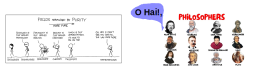
\includegraphics[width=1.1\textwidth]{images/xkcd-purity-w-philosophers}
      \end{overprint}
      
      {\tiny \href{https://xkcd.com/435/}{xkcd (Randall Monroe): Purity}}

\end{frame}
%%%%%%%%%%%%%%%%%%%%%%%%%%%%%%%%%%%%%%
\begin{frame}{Data, Theoretical Models, and Uncertainty}

\begin{columns}[T]
    \column{0.55\textwidth}
    \begin{itemize}
    \item ``dots'' ({\em measurement values}) are the job of the experimental physicist
    \item developing a ``line'' ({\em theoretical/mathematical model}) is the job of a theoretical physicist
    \item Each dot should actually have ``bars'' to indicate the {\em uncertainty} of each measurement
    \item A ``good'' theory is the simplest line that goes through the dots, taking into account the uncertainties
    \end{itemize}
    \column{0.45\textwidth}
      \includegraphics[width=\textwidth]{images/xkcd_curve-fitting}\\
      {\tiny \href{https://xkcd.com/2048/}{xkcd: Curve-Fitting}}
 \end{columns}
 

\end{frame}
%%%%%%%%%%%%%%%%%%%%%%%%%%%%%%%%%%%%%%
\begin{frame}{What is Physics: Sub-disciplines}

      \begin{overprint}
      \onslide<1>\includegraphics[width=\textwidth]{images/map-of-physics-walliman}
      \onslide<2>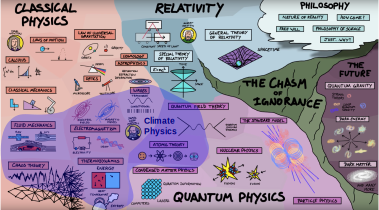
\includegraphics[width=\textwidth]{images/map-of-physics-walliman_w-climate-overlay}
      \end{overprint}
      
{\tiny \href{https://www.informationisbeautifulawards.com/showcase/1793-the-map-of-physics}{``The Map of Physics'' by Dominic Walliman} --- \href{https://www.youtube.com/watch?v=ZihywtixUYo}{2016 youtube video}}

\end{frame}
%%%%%%%%%%%%%%%%%%%%%%%%%%%%%%%%%%%%%%
\begin{frame}{Thermodynamics: Energy, Temperature, and Equilibrium}

\begin{center}
\begin{minipage}{0.8\linewidth}
\includegraphics[width=\textwidth]{images/temperature-equilibrium_hyperphysics}\\[-10pt]
\makebox[\textwidth][r]{
\tiny From \href{http://hyperphysics.phy-astr.gsu.edu/hbase/thermo/temper2.html}{{\em Hyperphysics --- A More General View of Temperature}}
}
\end{minipage}
\end{center}
%

\begin{itemize}
\item The {\em internal energy} of an object is the random ``thermal'' motion of its constituent particles.
\item {\em Temperature} is a measure of (proportional to) that energy
\item {\em Thermal contact} between two objects at different temperatures will eventually result in a common temperature ({\em thermal equilibrium})
\end{itemize}

\end{frame}
%%%%%%%%%%%%%%%%%%%%%%%%%%%%%%%%%%%%%%
\begin{frame}{Temperature Scales}

There are three common units of temperature.

\begin{center}
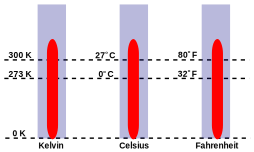
\includegraphics[width=0.8\textwidth]{images/temperature-scales}
\end{center}

\begin{itemize}
\item The first (Kelvin) is the physicist's standard unit
\item The last (Fahrenheit) is just weird, but comfortable
\item \underline{We will primarily use the second (Celsius)}
\end{itemize}

\end{frame}
%%%%%%%%%%%%%%%%%%%%%%%%%%%%%%%%%%%%%%
\begin{frame}{Thermometers}

There are three common units of temperature.

\begin{center}
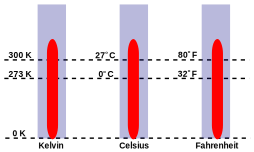
\includegraphics[width=0.8\textwidth]{images/temperature-scales}
\end{center}

\begin{itemize}
\item The first (Kelvin) is the physicist's standard unit
\item The last (Fahrenheit) is just weird, but comfortable
\item \underline{We will primarily use the second (Celsius)}
\end{itemize}

\end{frame}
%%%%%%%%%%%%%%%%%%%%%%%%%%%%%%%%%%%%%%
\begin{frame}{Climate Change is (pretty) {\em Recent}}


\begin{center}
\includegraphics[width=\textwidth]{images/global-avg-temperature-1860-present_may-2025-report_BEST}
\end{center}
\vspace{-0.5cm}
\hfill{\tiny Image and data From \href{https://berkeleyearth.org/may-2025-temperature-update/}{Berkeley Earth May 2025 update}}

{\small
\begin{itemize}
\item Note: {\em uncertainty} on each point and temperature {\em anomaly}
\item Temperature increase is outside uncertainty, but perhaps just {\em natural variation}?
\end{itemize}
}
\end{frame}
%%%%%%%%%%%%%%%%%%%%%%%%%%%%%%%%%%%%%%
\begin{frame}{Paleo-record of temperature (proxies)}

Looking at 4000 years of (proxy) temperature measurements\ldots

\vspace{1cm}

 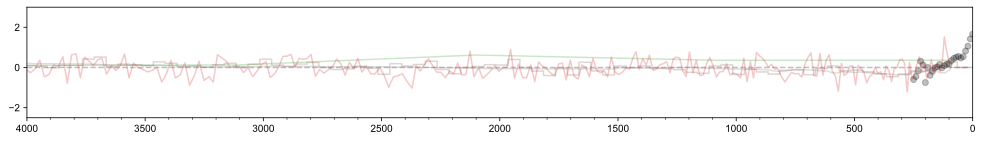
\includegraphics[width=1.05\textwidth]{images/row4_4kya}


\end{frame}
%%%%%%%%%%%%%%%%%%%%%%%%%%%%%%%%%%%%%%
\begin{frame}{This week in Discussion...}

\begin{center}
\includegraphics[width=\textwidth]{images/timescales-of-earth-and-temperature}
\end{center}

(Proxy) Temperature record over the history of the Earth

\end{frame}
\end{document}
